\chapter{Zahlenfolgen, Zahlenreihen, Konvergenz}

Der moderne Grenzwertbegriff stellt die Grundlage der Infinitesimalrechnung dar. In diesem Kapitel betrachten wir zuerst Zahlenfolgen und Reihen, definieren dann Konvergenz sowie Grenzwert und lernen abschließend einige wichtige Regeln zur Konvergenz und Grenzwertbestimmung kennen.

Um die Wichtigkeit zu illustrieren, warum eine exakte Definition der Konvergenz notwendig ist, sei Zenons Paradoxon von Achilles und der Schildkröte angeführt. \emph{Zeno of Elea} (etwa 500 BC) hat dieses Paradoxon angeführt, um zu zeigen, dass der naive Begriff von Wandel und Bewegung nur eine Illusion wäre. Zur besseren Veranschaulichung wählen für die folgende Erklärung (willkürlich gewählte) Größenabgaben. In dem Paradox nun veranstalten Achilles und eine Schildkröte ein Wettrennen, wie in Abbildung \ref{fig:ZenoAchilles} dargestellt. Achilles ist in der Lage, mit einer Geschwindigkeit von $25\ukmh$ zu rennen, während die Schildkröte nur $5\ukmh$ schafft. Der Fairness halber erhält die Schildkröte daher einen Vorsprung von $100\ukm$. Die Frage ist nun, wann Achilles die Schildkröte überholt. Der geläufige physikalische Ansatz wäre, ein Koordinatensystem zu definieren, die Bewegungsgleichungen beider Wettläufer aufzustellen und den Schnittpunkt zu berechnen. Zenon argumentiert allerdings wie folgt:

\begin{enumerate}
	\item Damit Achilles die Schildkröte überholen kann, muss er zunächst den Vorsprung von $100\ukm$ aufholen. Dazu benötigt er $4$ Stunden.
	\item In diesen $4$ Stunden allerdings ist die Schildkröte bereits $20\ukm$ weiter gekrochen.
	\item Also muss Achilles im nächsten Schritt diese $20\ukm$ Vorsprung aufholen, wozu er $0.8$ Stunden benötigt. Aber nun hat die Schildkröte bereits einen neuen Vorsprung erhalten.
	\item Egal, wie oft Achilles also den Vorsprung aufholt, um die Schildkröte zu überholen, müsste er unendliche viele Vorsprünge aufholen. Also holt Achilles die Schildkröte nie ein, um kann sie somit auch nicht überholen.
\end{enumerate}

Wie lässt sich dieses Paradoxon auflösen? Der Fehler, den Zenon hier begeht, besteht darin, dass Achilles zum Aufholen "unendlich" vieler Vorsprünge auch "unendlich" viel Zeit benötigt. Dies ist aber bei einer genauen Betrachtung mithilfe eines exakten Grenzwertbegriffs nicht der Fall, wie wir auch in einer Übungsaufgabe nachweisen werden.

\begin{figure}
	\centering
	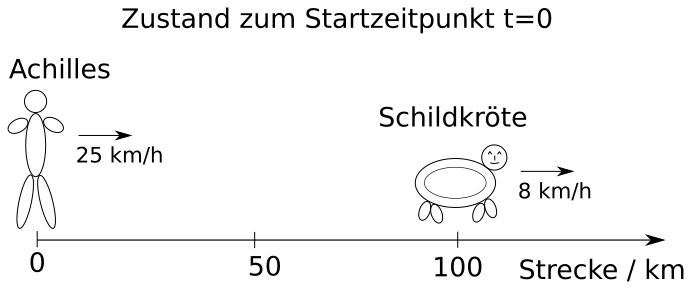
\includegraphics[width=0.75\textwidth]{./svg/zeno-achilles.png}
	\caption[Zenos Paradoxon des Wettrennens]{Zenos Paradoxon von dem Wettrennen zwischen Achilles und der Schildkröte}
	\label{fig:ZenoAchilles}
\end{figure}

\section{Zahlenfolgen}

Bevor wir den Begriff der Konvergenz näher definieren können, benötigen wir zuerst ein Verständnis von Zahlenfolgen.

\begin{definition}{Unendliche Zahlenfolge}{UnlimitSeq}
	Eine unendliche Zahlenfolge ist gegeben, wenn jeder natürlichen Zahl $n \ge 0$  genau eine (meist reelle) Zahl $a_n\in\R$ zugeordnet wird. $a_n$ heißt das $(n+1)$-te Glied der Zahlenfolge.
\end{definition}

\begin{definition}{Endliche Zahlenfolge}{LimitSeq}
	Besteht die Zuordnung nur für jede natürliche Zahl $n$ zwischen 0 und $N$ ($0 \le n \le N$), so spricht man von einer endlichen Zahlenfolge.
\end{definition}

Zahlenfolgen können also als Funktion $f: \N \to \R$ aufgefasst werden. Zur mathematischen Darstellung gibt es zwei Möglichkeiten:

\begin{enumerate}
	\item Explizite Darstellung: Der Wert des $n$.-ten Folgenglieds ist direkt gegeben.
	\item Implizite (rekursive) Darstellung: Der Wert des nächsten Folgengliedes ($n+1$) ist gegeben in Abhängigkeit eines oder mehrerer voriger Folgenglieder. Zudem ist ein Startwert für das erste oder die ersten Folgenglieder gegeben.
\end{enumerate}

Wir wollen uns diese beiden Möglichkeiten an zwei wichtigen Zahlenfolgen anschauen.

\begin{definition}{Arithmetische Zahlenfolge}{ArithSeq}
	Eine arithmetische Zahlenfolge ist gegeben, wenn in jedem Schritt das nächste Folgenglied durch Addition einer immer gleichen Konstanten zum vorigen Folgenglied bestimmt wird.
\end{definition}

\begin{definition}{Geometrische Zahlenfolge}{GeoSeq}
	Eine geometrische Zahlenfolge ist gegeben, wenn in jedem Schritt das nächste Folgenglied durch Multiplikation einer immer gleichen Konstanten mit dem vorigen Folgenglied bestimmt wird.
\end{definition}

Eine arithmetische Zahlenfolge beschreibt konstantes Wachstum und kann auch als lineare Funktion aufgefasst werden. Demgegenüber drückt eine geometrische Zahlenfolge exponentielles Wachstum, etwa die (initiale) Vermehrung von Bakterien in einer Petrischale. In Beispiel \ref{ex:ArithSeq} und \ref{ex:GeoSeq} sind diese beiden Zahlenfolgen anhand eines konkreten Beispiels in beiden Darstellungsformen zu sehen.

\begin{example}{Darstellung einer arithmetischen Zahlenfolge}{ArithSeq}
	Die arithmetische Zahlenfolge der ungeraden Zahlen beginnt mit $(a_n) = 1, 3, 5, 7, 9, ...$. Das Zahlenfolgenglied für $n=0$ ist $a_0=1$. Für $n=1$ ist $a_1=3$, für $n=2$ ist $a_2=5$. Wir erkennen sofort,
dass ein Folgenglied immer um $2$ größer ist als das vorige. Die rekursive Darstellung lautet somit also $a_{n+1} = a_n + 2$ mit dem Startwert $a_0 = 1$.  Wenn wir es nun noch schaffen, eine Formel für $a_n$ in Abhängigkeit von $n$ zu finden, haben wir auch die explizite Darstellung gefunden: $a_n = 2n+1$.
\end{example}

\begin{example}{Darstellung einer geometrischen Zahlenfolge}{GeoSeq}
	Analoges gilt für die geometrischen Zahlenfolgen. Beispielsweise ist $(a_n) = 1, \frac{1}{2}, \frac{1}{4}, \frac{1}{8}, \frac{1}{16}, ...$ eine geometrische Zahlenfolge. Jedes Folgenglied ergibt sich, indem das
vorige Folgenglied halbiert wird. Damit können wir die rekursive Darstellung angeben als $a_{n+1} = \frac{1}{2}a_n$ mit dem Startwert $a_0=1$. Für die explizite Darstellung erhalten wir nach etwas Nachdenken $a_n = {\frac{1}{2}}^n$. Wichtig zu betonen ist hier, dass es keine allgemein gültige Vorgehensweise gibt, die rekursive Darstellung in die explizite Darstellung umzuwandeln, hier ist wie in vielen Teilen der Mathematik kreatives Nachdenken erforderlich.
\end{example}

\begin{figure}
	\centering
	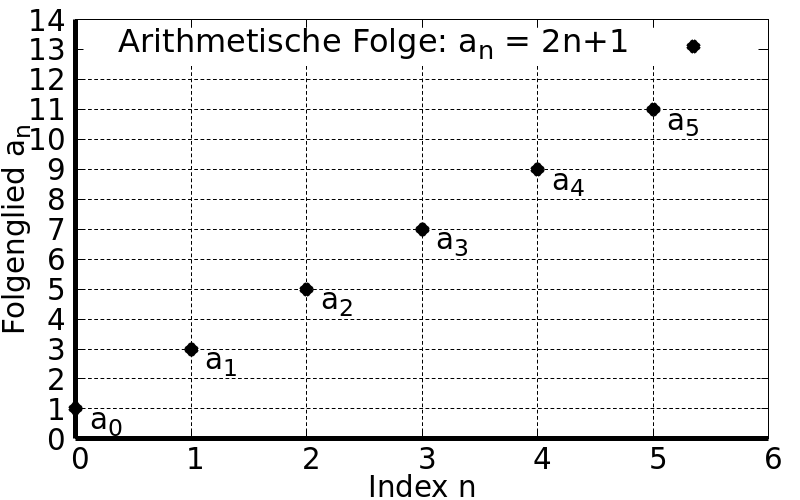
\includegraphics[width=0.8\textwidth]{./gnuplot/example-arithmetic-series.png}
	\caption[Arithmetische Folge]{Graphische Darstellung der arithmetischen Folge aus \ref{ex:ArithSeq}}
	\label{fig:ExArithSeq}
\end{figure}

\begin{figure}
	\centering
	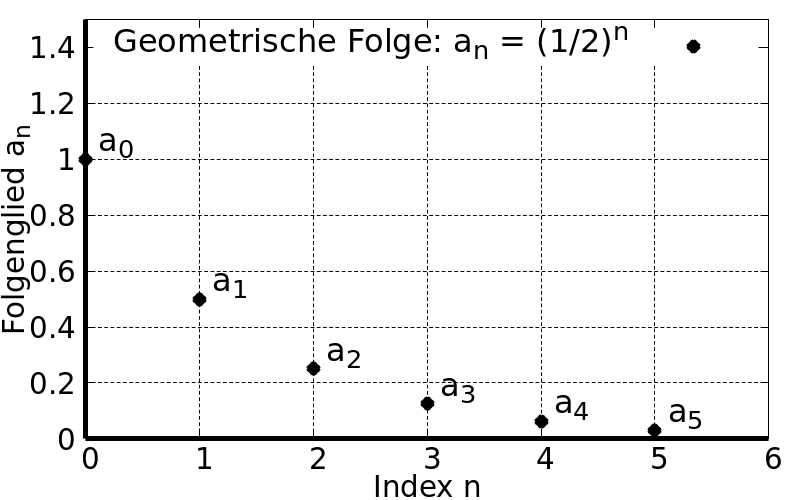
\includegraphics[width=0.8\textwidth]{./gnuplot/example-geometric-series.png}
	\caption[Geometrische Folge]{Graphische Darstellung der geometrischen Folge aus \ref{ex:GeoSeq}}
	\label{fig:ExGeoSeq}
\end{figure}

Wie in Abbildung \ref{fig:ExArithSeq} und \ref{fig:ExGeoSeq} dargestellt, lässt sich eine Zahlenfolge auch in einem Diagramm darzustellen. Hierbei ist zu beachten, dass nur Punkte, aber keine durchgehenden Linien eingezeichnet werden dürfen - denn der Definitionsbereich besteht nur aus den natürlichen Zahlen. Ebenfalls diesen beiden Abbildungen lässt sich entnehmen, dass Zahlenfolgen unterschiedlich verlaufen können. Die arithmetische Reihe steigt ohne Grenzen an, die geometrische Reihe $(a_n) = (\frac{1}{2})^n$ fällt und nähert sich immer weiter der $0$ an. Dies gibt Anlass, zwei wichtige Eigenschaften von Zahlenfolgen zu definieren.

\begin{definition}{Monotonie einer Zahlenfolge}{MonoSeq}
	Eine Zahlenfolge $(a_n)$ heißt \textbf{streng monoton wachsend}, wenn jedes Glied größer ist als das vorige, also $\forall n \in\N: a_{n+1} > a_n$ gilt. Analog heißt die Zahlenfolge \textbf{streng monoton fallend}, wenn jedes Glied kleiner ist als das vorige, also $\forall n \in\N: a_{n+1} < a_n$ gilt. Gilt nur $a_{n+1} \ge a_n$ beziehungsweise $a_{n+1} \le a_n$, so spricht man nur von einer \textbf{monoton steigenden} beziehungsweise \textbf{monoton fallenden} Folge (ohne dem Wörtchen "streng").
\end{definition}

\begin{definition}{Beschränktheit einer Zahlenfolge}{BoundSeq}
	Eine Zahlenfolge $(a_n)$ heißt \textbf{nach unten beschränkt}, wenn alle ihre Glieder überhalb einer unteren Grenze liegen, das heißt, wenn es ein $L\in\R$ gibt, sodass $\forall n \in\N: L \ge a_n$ gilt. $L$ heißt dann untere Schranke (lower bound) der Zahlenfolge, geschrieben als $L = \inf a_n$ (Infimum).

	Eine Zahlenfolge $(a_n)$ heißt \textbf{nach oben beschränkt}, wenn alle ihre Glieder unterhalb einer oberen Grenze liegen, das heißt, wenn es ein $U\in\R$ gibt, sodass $\forall n \in\N: L \le a_n$ gilt. $L$ heißt dann obere Schranke (lower bound) der Zahlenfolge, geschrieben als $U = \sup a_n$ (Supremum).
\end{definition}

Anmerkung: Manchmal betrachtet man auch nur die Beschränktheit einer Zahlenfolge ohne die ersten $N$ Glieder und schreibt dann $\inf\limits_{n \ge N} a_n$ beziehungsweise $\sup\limits_{n \ge N} a_n$.

\begin{example}{Eigenschaften der arithmetischen und geometrischen Zahlenfolge}{ArithGeoProp}
	Die arithmetische Zahlenfolge $a_{n+1} = a_n + C, a_0 = k, C > 0$ ist streng monoton steigend, denn $a_{n+1} > a_n$ ist äquivalent zu $a_n + C > a_n$ und weiter $C > 0$, was nach Voraussetzung eine wahre Aussage ist. Weiterhin ist sie nicht nach oben beschränkt (\textbf{unbeschränkt}), da für jede noch so große Zahl $U > 0$ sich durch Umstellung der expliziten Darstellung ein Folgenglied $n'$ finden lässt, sodass $a_{n'} > U$ gilt. Allerdings ist sie nach unten beschränkt, dass alle Glieder größer oder gleich dem Startwert $k$ sind.

	Analog findet man für arithmetische Zahlenfolgen mit $C<0$, dass sie monoton fallend, nach oben beschränkt und nach unten unbeschränkt ist. Für $C=0$ erhält man die sogenannte konstante Folge, welche sowohl monoton steigend als auch fallend ist (aber nicht streng), und sowohl nach oben als auch nach unten beschränkt ist.

	Für die geometrische Zahlenfolge $a_{n+1} = q \cdot a_n, a_0 = p, 0 < q < 1, p > 0$ stellt wir zuerst fest, dass alle ihre Glieder positiv sind. Sie ist streng monoton fallend, denn $a_{n+1} < a_n$ ist äquivalent zu $q \cdot a_n < a_n$ und weiter (da $a_n$ positiv) $q < 1$, was nach Voraussetzung eine wahre Aussage ist. Sie ist nach oben beschränkt, da sie monoton fallend ist. Weiterhin ist sie auch nach unten beschränkt, da alle Folgeglieder positiv sind (und damit $L=0$ eine untere Schranke darstellt).
\end{example}

\section{Konvergenz und Grenzwertbegriff}

Eine weitere Eigenschaft von fundamentaler Bedeutung ist das sogenannte Konvergenzverhalten einer Zahlenfolge. An dem Beispiel der geometrischen Folge $(\frac{1}{2})^n$ in Abbildung \ref{fig:ExGeoSeq} haben wir bereits gesehen, dass sich diese scheinbar immer weiter der $0$ anzunähern scheint, ohne diese jemals (im Endlichen) zu erreichen. Diese Idee, dass eine Folge sich einem Grenzwert immer weiter nähert, wird durch die folgende Definition präzisiert.

\begin{definition}{Konvergenz und Grenzwert}{Convergence}
	Eine Folge $(a_n)$ heißt \textbf{konvergent} mit dem \textbf{Grenzwert} $\alpha$, wenn der Abstand der Folgenglieder zum Grenzwert beliebig klein wird und klein bleibt. Andernfalls heißt sie \textbf{divergent}.

	$\forall \varepsilon > 0 \exists n_0\in\N: \forall n > n_0 : |a_n - \alpha| < \varepsilon$

	Man schreibt dann: $\lim\limits_{n\to\infty} a_n = \alpha$.
\end{definition}

Anders formuliert kann man auch sagen, die Folge $(a_n)$ heißt konvergent mit dem Grenzwert $\alpha$, wenn man zu jedem noch so kleinen Abstand zum Grenzwert (bezeichnet mit $\varepsilon$) immer eine Position in der Zahlenfolge finden kann, sodass alle Folgenglieder rechts von dieser Position innerhalb dieses Abstands liegen. Visuell wird diese Definition durch Abbildung \ref{fig:VisLimit} illustriert.

\begin{figure}
	\centering
	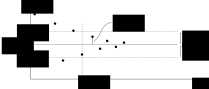
\includegraphics[width=0.8\textwidth]{./svg/definition-convergence.png}
	\caption{Graphische Veranschaulichung des Grenzwertbegriffs}
	\label{fig:VisLimit}
\end{figure}

In Beispiel \ref{ex:ConvGeoSeq} und \ref{ex:ConvConstSeq} wird gezeigt, wie man anhand dieser Definition nachweisen kann, ob eine Folge konvergent ist und welchen Grenzwert sie hat. Ebenfalls wie in Beispiel \ref{ex:ConvAltSeq} kann man zeigen, dass eine Folge divergent ist. Für die praktische Bestimmung von Grenzwerten ist diese Definition sehr umständlich, wir werden daher in Kürze Rechenregeln kennen lernen, um die Berechnung von Grenzwerten zu vereinfachen.

\begin{example}{Konvergenz der geometrischen Folge}{ConvGeoSeq}
	Wir betrachten noch einmal die geometrische Folge $a_n = (\frac{1}{2})^n$. Wir vermuten, dass $\alpha=0$ der Grenzwert ist. Um dies zu beweisen, benutzen wir die obige Definition. Sei $\varepsilon>0$. Wir müssen
	nun ein $n_0$ finden, sodass $|a_n-\alpha|=(\frac{1}{2})^n < \varepsilon$ gilt, wenn $n > n_0$. Durch Umstellen der Ungleichung erhalten wir $n > \log_{1/2}(\varepsilon)$ (man beachte, dass sich das Ungleichheitszeichen umkehrt, da $\log_{1/2}$ eine monoton fallende Abbildung ist). Die Ungleichung ist also erfüllt, solange wir Folgenglieder $a_n$ betrachten, wo $n$ größer als $\log_{1/2}(\varepsilon)$ ist. Abschließend setzen wir $n_0 = \floor{\log_{1/2}(\varepsilon)}$, wobei die Klammer mit dem unteren Hacken für die Operation "Abrunden" stehen. Damit können wir schreiben:

	$$
	\forall \varepsilon > 0 \exists n_0 = \floor{\log_{1/2}(\varepsilon)} : \forall n > n_0 : |a_n - 0| < \varepsilon
	$$

	Also ist die geometrische Folge $a_n = (\frac{1}{2})^n$ konvergent und hat den Grenzwert $\alpha=\lim\limits_{n\to\infty}(\frac{1}{2})^n=0$.
\end{example}


\begin{example}{Konvergenz der konstanten Folge}{ConvConstSeq}
	Die konstante Folge $a_n = 1$ ist ebenfalls konvergent und hat den Grenzwert $\alpha = 1$, denn für den Abstand gilt $|a_n-\alpha|=|1-1|=0<\varepsilon$. Wir erkennen an diesem Beispiel, dass es nicht von Relevant ist, ob die Folgenglieder den Grenzwert erreichen oder nicht -- entscheidend ist lediglich der Abstand zum Grenzwert, und dieser kann auch $0$ betragen kann.
\end{example}


\begin{example}{Divergenz der alternierenden Folge}{ConvAltSeq}
	Die Folge $a_n = (-1)^n$ mit den Gliedern $1,-1,1,-1,...$ heißt alternierende Folge. Diese ist zwar nach oben und unten beschränkt (durch $L=-1$ und $U=1$), besitzt allerdings keinen Grenzwert. Wählt man etwa $\alpha=1$, erhält man für den Abstand $(d_n) = |a_n-\alpha|=(-1)^n-1| = (0, 2, 0, 2, 0, 2)$. Ist $\varepsilon$ nun genügend klein, etwa $0.5$, so findet man immer wieder ein Folgenglied, dessen Abstand zum Grenzwert größer ist als $\varepsilon$. Egal, welchen Grenzwertkandidaten man wählt, es ist nicht möglich, den Abstand zum Grenzwertkandidaten beliebig klein zu halten.
\end{example}

Ist eine Folge nicht konvergent, so heißt Sie wie erwähnt divergent und besitzt folglich auch keinen Grenzwert. Nun gibt es eine besondere Art der Divergenz, bei der man gelegentlich auch davon spricht, der Grenzwert sei $\pm\infty$. Diese Aussage ist immer im Sinne der folgenden Definition zu verstehen:

\begin{definition}{Bestimmte Divergenz}{Divergence}
	Eine Folge heißt \textbf{bestimmt divergent} gegen $+\infty$ ($-\infty$), falls die Folgenglieder beliebig groß (klein) werden und auch groß (klein) bleiben.

	$$
	\forall R > 0 \exists n_0\in\N: \forall n > n_0 : a_n > R
	$$

	$$
	\forall R < 0 \exists n_0\in\N: \forall n > n_0 : a_n < R
	$$

	Man schreibt dann auch $\lim\limits_{n\to\infty}a_n = +\infty$ beziehungsweise $\lim\limits_{n\to\infty}a_n = -\infty$.
\end{definition}


\begin{example}{Divergenz der arithmetischen Folge}{DivArithSeq}
	Die arithmetische Folge $a_n=2n+1$ ist bestimmt divergent gegen $\infty$. Aus $2n+1 > R$ erhalten wir $n > \frac{R-1}{2}$ Wählen wir nun $n_0 = \floor{\frac{R-1}{2}}$, so können wir schreiben:

	$$
	\forall R > 0 \exists n_0 = \floor{\frac{R-1}{2}}: \forall n > n_0 : a_n > R
	$$

	Es ist also $\lim\limits_{n\to\infty} 2n+1 = \infty$.
\end{example}


\section{Reihen}

Bei einer Reihe handelt es sich um eine ganz bestimmte Form einer Zahlenfolge, die eine eigene Bezeichnung erhalten hat, da sie in der Praxis häufig vorkommt. Etwa wird der von Achilles aufgeholte Vorsprung der Schildkröte in jedem Schritt durch eine geometrische Zahlenfolge beschrieben. Der gesamte zurückgelegte Weg ergibt sich durch Addition der einzelnen Teilwege und stellt eine geometrische Reihe dar.

\begin{definition}{Begriff der Reihe}{Series}
	Eine \textbf{Reihe} $(s_n)$ entsteht durch Summation der Glieder einer Zahlenfolge. Die Summe $s_n=\sum\limits_{i=0}^n a_i$ der ersten $(n+1)$-Glieder heißt \textbf{Partialsumme}. Der Grenzwert der Partialsummen, falls existent, $s_\infty = \lim\limits_{n\to\infty}s_n$ heißt \textbf{unendliche Reihe}.
\end{definition}

Anhand der arithmetischen und geometrischen Folge und der daraus induzierten Reihe wird der Reihenbegriff in den Beispielen \ref{ex:PartSumArithSer} und \ref{ex:PartSumGeoSer} verdeutlicht.

\begin{example}{Partialsummen der arithmetischen Reihe}{PartSumArithSer}
	Die arithmetische Reihe $a_n = k\cdot n+m$ mit $k,m\in\R$ ist für $k \ne 0$ unbeschränkt, die unendliche Reihe wird daher nicht existieren. Die Partialsummen lauten $s_n = \sum\limits_{i=0}^n (ki+m)$. Durch Anwendung des Assoziativ- und Distributivgesetzes können wir dies umformen zu $\left(k\cdot\sum\limits_{i=0}^n i\right) + \left(\sum\limits_{i=0}^n m\right)$. Die rechte Summenbildung stellt lediglich die Addition der $(n+1)$ konstanten Zahlen $m$ dar und beträgt mithin $m\cdot(n+1)$.

	Für die linke Summe $\sum\limits_{i=0}^n i$ müssen wir die ersten $n$ natürlichen Zahlen aufaddieren. Hierzu bedienen wir uns eines Verfahrens, welches unter anderem durch \mention{Carl Friedrich Gauß} bekannt geworden ist. Um die Zahlen von $1$ bis $100$ zu addieren, teilte er die Summe auf in Paare: $1+100$, $2+99$, $3+98$, $4+97$ und so fort. Jedes Paar hat den Wert $101$, ingesamt gibt es $50$ Paare. Damit beträgt die Summe $50\cdot 101 = 5050$. Allgemein gilt, das wenn die Zahlen von $1$ bis $n$ zu addieren sind, es dann $n/2$-Paare mit jeweils dem Wert $n+1$ gibt und deren Summe $\frac{n(n+1)}{2}$ beträgt.

	Man beachte dabei den Fall, wenn $n$ ungerade ist, also ein ungerade Anzahl an Zahlen zu addieren ist. Dann gibt es nur $(n-1)/2$-Paare mit der Summe $(n+1)$ und die mittlere Zahl $(n+1)/2$ bleibt übrig. Letzlich beträgt die Summe somit ebenfalls $\frac{n-1}{2}(n+1)+\frac{n+1}{2} = \frac{n(n+1)}{2}$.

	Insgesamt gewinnen wir für die Partialsummen somit den Ausdruck:

	\begin{equation}
	  s_n = k \frac{n(n+1)}{2} + m\cdot(n+1) = \frac{k}{2}n^2 + \left(m+\frac{k}{2}\right)n + m
	\end{equation}

	Beispielsweise können wir anhand dieser Formel berechnen, dass die Summe der ungeraden Zahlen kleiner $100$ lautet

	$$
	  1+3+5+...+97+99 = \sum\limits_{n=0}^{49} 2n+1 = 2\frac{49\cdot 50}{2} + 50 = 2500
	$$
\end{example}

\begin{example}{Partialsummen der geometrischen Reihe}{PartSumGeoSer}
	Die geometrische Folge lautet $a_n = p \cdot q^n$ mit $p,q\in\R$. Um die Partialsummen $s_n = \sum\limits_{i=0}^n p\cdot q^i$ zu bestimmen, bedienen wir uns eines kleinen Umformungstricks. Die Partialsumme wird mit der konstanten $q$ multipliziert und von der ursprünglichen Partialsumme abgezogen, sodass sich fast alle Summanden aufheben:

	\begin{alignat*}{4}
		        s_n       &= p \cdot ( & q^0 + & q^1 + q^2 + q^3 + ... + q^n           &) \\
		q \cdot s_n       &= p \cdot ( &       & q^1 + q^2 + q^3 + ... + q^n + q^{n+1} &)
	\end{alignat*}
	\begin{alignat*}{1}
		s_n - q \cdot s_n &= p \cdot (1 - q^{n+1}) \\
          s_n \cdot (1-q) &= p \cdot (1 - q^{n+1})
	\end{alignat*}

	Die letzte Gleichung können wir nun direkt nach der gesuchten Partialsumme $s_n$ umstellen und erhalten:

	\begin{equation}
	  s_n = p \frac{1 - q^{n+1}}{1 - q}
	\end{equation}

	Mithilfe dieser Formel können wir nun beispielsweise die Summe aller Inversen von Zweierpotenzen berechnen:

	$$
	 1 + \frac{1}{2} + \frac{1}{4} + \frac{1}{8} + ... + \frac{1}{256} = \sum\limits_{n=0}^8 (\frac{1}{2})^n = \frac{1 - (1/2)^9}{1/2} = \frac{1022}{512} = \frac{511}{256}
	$$
\end{example}

\begin{example}{Grenzwert der geometrischen Reihe}{LimGeoSer}
    Die Partialsummen der geometrischen Reihe lauten $s_n = p \frac{1 - q^{n+1}}{1 - q}$. Für welche Werte von $p$ und $q$ konvergieren diese bei $n\to\infty$. Die meisten Terme in der Partialsumme sind unabhängig von $n$, der einzige von $n$ abhängige Term lautet $q^{n+1}$ und ist selbst wieder eine geometrische Folge. Diese konvergiert für $|q| < 1$ gegen $0$. Für $q=1$ ist die geometrische Reihe $1+1+1+\dots$ offensichtlich divergent. Somit ist die geometrische Reihe konvergent für $|q|<1$ und hat den Grenzwert:
    $$
        s_\infty = \lim\limits_{n\to\infty} \sum\limits_{i=0}^n p\cdot q^i = \frac{p}{1-q}
    $$
    Es ergibt sich also beispielsweise $1 + \frac{1}{2} + \frac{1}{4} + \frac{1}{8} + ... = \frac{1}{1/2} = 2$.
\end{example}

\section{Konvergenz von Folgen}

Wir haben bereits die formale Definition von Konvergenz kennengelernt. Auch haben wir gesehen, dass man zwar anhand dieser Definition Grenzwert bestimmen kann, dies meist aber nur recht umständlich möglich ist. Für die praktische Berechnung von Grenzwerten wollen wir uns daher noch einige Rechenregeln anschauen, welche die Rechenarbeit erleichtern.

Komplexe Terme sind durch Rechenoperationen aus einfacheren Termen aufgebaut. Zuerst benötigen wir die Grenzwerte einiger spezieller Terme. Diese seien im Folgenden ohne Beweis angegeben:

\begin{statement}{Grenzwerte einiger spezieller konvergenter Folgen}{LimSpecSeq}
	Die folgenden Folgen sind konvergent und haben den angegeben Grenzwert.
	\begin{alignat}{3}
		& \lim\limits_{n\to\infty} & \frac{1}{n^q}  & = 0, q > 0 \label{eq:LimitInv1nq} \\
		& \lim\limits_{n\to\infty} & q^n & = 0, |q| < 1 \\
		& \lim\limits_{n\to\infty} & \nroot{n}{n} & = 1 \\
		& \lim\limits_{n\to\infty} & \nroot{n}{q} & = 1, q > 0 \\
		& \lim\limits_{n\to\infty} & \frac{a^n}{n!} & = 0, a \in \R \label{eq:LimitPowerFactorial} \\
		& \lim\limits_{n\to\infty} & \left(1+\frac{1}{n}\right)^n & = e \label{eq:LimitExp}
	\end{alignat}
\end{statement}

Ein wichtiger Satz, der manchmal bei schwierigen Grenzwerten hilft, ist das sogenannte \emph{Sandwich-Kriterium}. Schafft man es zu zeigen, dass eine Folge zwischen zwei anderen Folgen liegt, so muss auch der Grenzwert der Folgen zwischen den Grenzwerten der anderen beiden Folgen liegen. Haben diese beiden Folgen den gleichen Grenzwert, kennt man damit den Grenzwert der zu untersuchenden Folge.

\begin{statement}{Sandwich-Kriterium}{SandwichTheo}
	Gegeben sei eine Folge $(a_n)$. Gibt es zwei konvergente Folgen $(l_n)$ und $(u_n)$, die beide gegen den gleichen Grenzwert $\alpha$ konvergieren, und gilt ab einem bestimmten Folgenglied $n_0$ die Ungleichung $l_n \le a_n \le u_n, n \ge n_0$, dann konvergiert auch die Folge $a_n$ gegen $\alpha$.
\end{statement}

\begin{example}{Anwendung des Sandwich-Kriteriums}{SandwichTheo}
	Gesucht ist der Grenzwert der Folge $a_n = \frac{1}{n^2}\sin(n)$. Von den elementaren Eigenschaften der Sinusfunktion wissen wir, dass gilt $-1\le\sin(n)\le 1$. Wählen wir nun $l_n = -\frac{1}{n^2}$ und $u_n = \frac{1}{n^2}$, so gilt $l_n \le a_n \le u_n$. Die Folge $a_n$ wird also durch die zwei Folgen $(l_n)$ und $(u_n)$ eingeschachtelt. Für diese beiden Folgen gilt nach \ref{eq:LimitInv1nq} $\lim\limits_{n\to\infty} \pm\frac{1}{n^2} = 0$. Nach dem Sandwich-Kriterium \ref{stmt:SandwichTheo} folgt somit $\lim\limits_{n\to\infty} \frac{1}{n^2}\sin(n) = 0$.
\end{example}

Folgende Regeln gelten, wenn eine neue Folge durch Addition oder Multiplikation der Glieder zweier anderer Folgen gebildet wird:

\begin{statement}{Grenzwertregeln für zusammengesetzte Folgen}{CombSeqLimit}
	Seien $(a_n), (b_n), (c_n)$ konvergente Zahlenfolgen mit jeweils dem Grenzwert $a, b, c$ und $c_n, c \ne 0$. Sei zudem $c \in \R$ eine Konstante und $f: \R\to\R$ eine stetige Funktion. Dann gelten die folgenden Rechenregeln für Grenzwerte:

	\begin{alignat}{2}
		& \lim\limits_{n\to\infty}(a_n \pm b_n) & = a + b \label{eq:LimSum} \\
		& \lim\limits_{n\to\infty}(a_n \cdot b_n) & = a \cdot b \label{eq:LimProd} \\
		& \lim\limits_{n\to\infty}(a_n / c_n) & = a / c \label{eq:LimQuot} \\
		& \lim\limits_{n\to\infty}(c \cdot a_n) & = c \cdot a \label{eq:LimCoeff} \\
		& \lim\limits_{n\to\infty}(f(a_n)) & = f(a)	\label{eq:LimFun}
	\end{alignat}
\end{statement}

Gleichung \ref{eq:LimSum} und \ref{eq:LimProd} sagen aus, dass bei einem Grenzwert von Summen und Produkten die Grenzwerte der Summanden und Faktoren einzeln betrachtet werden können. Gleichung \ref{eq:LimCoeff} ist eine einfache Konsequenz aus \ref{eq:LimProd}. Die letzte Gleichung \ref{eq:LimFun} sagt aus, dass bei Anwendung einer (stetigen) Funktionen auf die Glieder einer Zahlenfolge die Grenzwertbildung in das Funktionsargument gezogen werden kann.	Übrig bleibt Gleichung \ref{eq:LimQuot}, welche analog zu den ersten beiden Gleichungen aussagt, dass auch bei einer Quotientenbildung die Grenzwerte von Dividend und Divisor einzeln betrachtet werden können. Allerdings muss hier die wichtige Einschränkung beachtet werden, dass die Glieder und der Grenzwert des Divisors ungleich $0$ sind, da die Division durch $0$ nicht erklärt ist. Nun gibt es aber speziell Folgen von Quotienten, wo die Glieder des Divisors zwar ungleich $0$ sind, der Grenzwert des Divisors aber nicht.

In \ref{ex:CombSeqLimit} sind einige für die ersten vier Regeln zusammengefasst.

\begin{example}{Anwendung der Grenzwertregeln für zusammengesetzte Folgen}{CombSeqLimit}
    \begin{itemize}
        \item $\lim\limits_{n\to\infty} \frac{n^2+1}{n^3} = \lim\limits_{n\to\infty} \left(\frac{1}{n} + \frac{1}{n^3}\right) = 0 + 0 = 0$ \\
        \item $\lim\limits_{n\to\infty} \frac{n-2}{n^2-3n+2} = \lim\limits_{n\to\infty} \frac{n(1-2/n)}{n^2(1-3/n+2/n^2)} = \lim\limits_{n\to\infty} \frac{1}{n} \cdot \frac{1-2/n}{1-3/n+2/n^2} = 0 \cdot \frac{1-0}{1-0+0} = 0$ \\
        \item $\lim\limits_{n\to\infty} \frac{n^2+1}{n-1} = \lim\limits_{n\to\infty} \frac{n^2(1+2/n^2)}{n(1-1/n)} = \lim\limits_{n\to\infty} n \cdot \frac{1+2/n^2}{1-1/n} = \infty $
        \item $\lim\limits_{n\to\infty} \frac{4n^3+2n}{7n^3-4n^2} = \lim\limits_{n\to\infty} \frac{n^3(4+2/n^2)}{n^3(7-4/n)} = 1 \cdot \frac{4+0}{7-0} = \frac{4}{7}$
    \end{itemize}
\end{example}

Die Anwendung der Rechenregel \ref{eq:LimFun} wird in Beispiel \ref{ex:LimFun} verdeutlicht.

Um auch Grenzwerte von Quotienten berechnen zu können, wo der Divisor gegen $0$ konvergiert, hilft die folgende Aussage. Dazu benötigen wir noch zwei Definitionen.

Bisher haben wir nur Grenzwerte betrachtet, wo $n$ gegen $\infty$ lief. Es ist nun aber so, dass man Grenzwerte nicht nur für Folgen, sondern auch für Funktionen betrachten kann, wenn das Funktionsargument sich einem bestimmten Wert (nicht zwingend $\infty$) nähert.

\begin{definition}{Grenzwert einer Funktion}{LimFun}
    Sei $f: \R^n \to \R$ eine Funktion, welche $n$-dimensionale Punkte auf reelle Zahlen abbildet, und sei $x_0\in\R^n$ eine Stelle des Definitionsbereichs. Die Zahl $\alpha\in\R$ heißt Grenzwert von $f$ gegen $x_0$, wenn es für jede noch so kleine Epsilon-Kugel um $\alpha$ eine Delta-Kugel um $x_0$ gibt, sodass die Funktionswerte der Delta-Kugel in der Epsilon-Kugel liegen.
    $$
        \forall \varepsilon > 0 \exists \delta > 0 : f(S_\delta(x_0)) \subset S_\varepsilon(\alpha)
    $$
    Man schreibt dann $\lim\limits_{x\to x_0} = \alpha$.
\end{definition}

Graphisch ist diese Definition dargestellt in Abbildung \ref{fig:LimFun} und bedeutet anschaulich, dass kleine Änderungen des Arguments immer nur kleine Änderungen des Funktionswerts zur Folge haben. Äquivalent zu dieser Definition ist, dass für jede gegen $x_0$ konvergent Folgen $a_n$ auch die Folge $f(a_n)$ der Funktionswerte gegen $\alpha$ konvergieren muss. Wenn der Grenzwert existiert, dann kann man ihn dadurch bestimmen, indem man die Grenzwertbildung für die einzelnen Variablen ($x_1, x_2, \dots$) der Reihe nach ausführt.

\begin{figure}
    \centering
    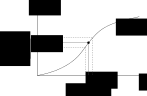
\includegraphics[width=0.55\textwidth]{./svg/definition-convergence-point}
    \caption[Grenzwert einer Funktion]{Grenzwert einer Funktion an einer Stelle $x_0$}
    \label{fig:LimFun}
\end{figure}

Die Grenzwertregeln, die wir bisher kennengelernt haben, sind analog auch auf Grenzwerte von Funktionen übertragbar.

\begin{example}{Grenzwertregeln für Grenzwert einer Funktion}{LimFunSumQuot}
    Auf $\lim\limits_{x\to 0} \frac{x^2+x+2}{x^3+1}$ lassen sich analog die Grenzwertregeln \ref{eq:LimSum} und \ref{eq:LimQuot} anwenden und man erhält: $\frac{0^2+0+2}{0^3+1} = 2$.
\end{example}

\begin{example}{Nichtexistenz des Grenzwerts einer einstelligen Funktion}{CheckLimUnivarFun}
    Die einstellige Funktion $f: x \mapsto \sin(1/x)$ hat keinen Grenzwert für $x \to 0$. Je nachdem, wir wir uns $0$ nähern, erhält man verschiedene Ergebnisse. Beispielsweise können wir die Folgen $a_n = \frac{2}{\pi+4\pi n}$ und $b_n = \frac{1}{\pi n}$ betrachten. Diese konvergieren beiden gegen $0$. Allerdings gilt für die Folgen der Funktionswerte:
    \begin{alignat}{1}
       \lim\limits_{n\to\infty} f(a_n) &= \lim\limits_{n\to\infty} \sin\left(1 / \frac{2}{\pi+4\pi n}\right) = \lim\limits_{n\to\infty} \sin(\frac{\pi}{2} + 2\pi n) = 1 \\
       \lim\limits_{n\to\infty} f(b_n) &= \lim\limits_{n\to\infty} \sin\left(1 / \frac{1}{\pi n}\right) = \lim\limits_{n\to\infty} \sin(\pi n) = 0 \\
    \end{alignat}
    Wir erhalten verschiedene Werte, somit existiert der Grenzwert nicht.
\end{example}

\begin{example}{Nichtexistenz des Grenzwerts einer mehrstelligen Funktion}{CheckLimMultivarFun}
    Die mehrstellige Funktion $f: (x,y) \mapsto \frac{x^2-y^2}{x^2+y^2}$ hat keinen Grenzwert für $(x_0,y_0) \to (0,0)$. Je nachdem, auf welchem Weg wir uns $(0,0)$ annähern, erhalten wir verschiedene Grenzwerte. Wenn wir uns dem Koordinatenursprung etwa nähern, indem wir erst zur x-Achse $y=0$ gehen, erhalten wir:
    $$
    \lim\limits_{x\to 0} \lim\limits_{y\to 0} \frac{x^2-y^2}{x^2+y^2} = \lim\limits_{x\to 0} \frac{x^2}{x^2} = 1
    $$
    Andererseits gilt, wenn wir erst zur y-Achse $x=0$ gehen:
    $$
    \lim\limits_{y\to 0} \lim\limits_{x\to 0} \frac{x^2-y^2}{x^2+y^2} = \lim\limits_{y\to 0} \frac{-y^2}{y^2} = -1
    $$
    Wir erhalten verschiedene Werte, somit existiert der Grenzwert nicht.
\end{example}

\begin{statement}{Grenzwert gebrochenrationaler Funktionen}{LimRatFun}
    Aus den bisherigen Beispielen können wir die folgende allgemeine Regel ableiten, die für den Grenzwert eines Quotienten von Polynomen gilt:
    Sei $f(x) = \frac{p_n(x)}{q_m(x)}$ eine gebrochenrationale Funktion, also der Quotient zweier Polynome $p_n, q_m$ vom Grad $n$ und $m$. Der Grenzwert existiert, wenn der Grad des Zählerpolynoms nicht kleiner ist als der Grad des Nennerpolynoms. Es gilt:

    \begin{equation}
    \lim\limits_{x\to\infty}\frac{p_n(x)}{q_m(x)} = \lim\limits_{x\to\infty}\frac{a_0 + a_1 x + a_2 x^2 + ... + a_n x^n}{b_0 + b_1 x + b_2 x^2 + ... + b_n x^n} = \begin{cases}
    0 &\text{falls $n < m$} \\
    \frac{a_n}{b_m} &\text{falls $ n = m$} \\
    \pm \infty  &\text{falls $ n > m$}
    \end{cases}
    \end{equation}

    Das Vorzeichen für den letzten Fall ergibt sich aus dem Vorzeichen der höchsten Koeffizienten $a_n$ und $b_n$. Sind beide positiv oder negativ, divergiert $f$ bestimmt gegen $+\infty$. Haben sie verschiedenes Vorzeichen, divergiert $f$ bestimmt gegen $-\infty$.
\end{statement}

Für die nächste Grenzwertregel benötigen wir weiterhin noch das Konzept der sogenannten \emph{unbestimmten Ausdrücke}.

\begin{definition}{Unbestimmte Ausdrücke}{IndetForms}
	Wir sprechen von einem \textbf{unbestimmten Ausdruck}, wenn eine Zahlenfolge aus zwei mit einer Rechenoperation verknüpften konvergenten oder bestimmt divergenten Einzelfolgen besteht, die obigen Grenzwertregeln aber nicht anwendbar sind.

	Die \textbf{Form des unbestimmten Ausdrucks} erhält man, indem man die Grenzwerte der Einzelfolgen mit der Rechenoperation verknüpft aufschreibt.
\end{definition}

Einige Beispiele für solche unbestimmten Ausdrücke finden sich in \ref{ex:IndetForms}. An diesesr Stelle sei noch eine Anmerkung angebracht: Manchmal spricht man davon, dass $1/0$ "unendlich" sei. Dies ist so aber nicht korrekt. Zum einen ist ein Ausdruck der Form $1/0$ immer nur als unbestimmter Ausdruck zu verstehen. Zum zweiten verbirgt sich hinter einem unbestimmten Ausdruck immer ein Grenzwert. Nur, wenn jeder Grenzwert der Form $1/0$ konvergent (oder bestimmt divergent) mit dem gleichen Grenzwert wäre, ließe sich diese Aussage rechtfertigen. Nun ist aber $\lim\limits_{n\to\infty} \frac{1}{1/n} = \infty$ und $\lim\limits_{n\to\infty} \frac{1}{-1/n} = -\infty$, beide sind aber unbestimmte Ausdrücke der Form $1/0$. Gleiches gilt für den unbestimmten Ausdruck $0^0$ -- je nach Wahl der konkreten Zahlenfolgen erhält man hier verschiedene Grenzwerte.

\begin{example}{Unbestimmte Ausdrücke}{IndetForms}
	\begin{itemize}
		\item $\lim\limits_{x\to\infty} \frac{\sin(n)}{e^x}$ ist ein unbestimmter Ausdruck der Form $\frac{\infty}{\infty}$
		\item $\lim\limits_{x\to\infty} e^{-x} \cdot x^2$ ist ein unbestimmter Ausdruck der Form $0 \cdot \infty$.
		\item $\lim\limits_{x\to 0} x^x$ ist ein unbestimmter Ausdruck der Form $0 ^ 0$.
	\end{itemize}
\end{example}

Mit diesem Wissen lässt sich nun die nächste Rechenregel formulieren.

\begin{statement}{Regel von L'Hôpital}{HopitalRule}
	Seien $f,g: \R\to\R$ zwei differenzierbare Funktionen und ist $\lim\limits_{n\to x_0} \frac{f(x)}{g(x)}$ ein unbestimmter Ausdruck der Form $\frac{0}{0}$ oder $\frac{\infty}{\infty}$, dann gilt:

    \begin{equation}
        \lim\limits_{x \to x_0} \frac{f(x)}{g(x)} = \lim\limits_{x \to x_0} \frac{f'(x)}{g'(x)}
    \end{equation}

    Voraussetzung hierbei ist, dass der rechte Grenzwert existiert. Aus der Nichtexistenz des rechten Grenzwerts \textbf{darf nicht} auf die Nichtexistenz des ursprünglichen Grenzwerts geschlossen werden.
\end{statement}

\begin{example}{Anwendung der Regel von L'Hôpital}{HopitalRule}
    \begin{itemize}
        \item $\lim\limits_{x\to\infty} \frac{\ln(x)}{x^2} = \lim\limits_{x\to\infty} \frac{1/x}{2x} = \lim\limits_{x\to\infty} \frac{1}{2x^2} = 0$
        \item $\lim\limits_{x\to\infty} x \cdot \ln(x) = \lim\limits_{x\to\infty} \frac{\ln(x)}{1/x} = \lim\limits_{x\to\infty} \frac{1/x}{-1/x^2} = 0$
        \item $\lim\limits_{x\to\infty} \frac{\sin(x)}{x} = \lim\limits_{x\to\infty} \frac{\cos(x)}{1} = \cos(0) = 1$
    \end{itemize}
\end{example}

\begin{example}{Vertauschung von Grenzwert und Funktionsanwendung}{LimFun}
    Gesucht ist der Grenzwert $\alpha = \lim\limits_{x\to 0^+} x^x$. Dabei bedeutet $x\to 0^+$, dass nur nicht-negative Funktionsargumente betrachtet werden, da $x^x$ sonst nicht erklärt ist, dies nennt man auch \emph{rechtsseitiger Grenzwert}. Wir wenden den Logarithmus auf beide Seiten der Gleichung an, und machen dann von der Rechenregel \ref{eq:LimFun} Gebrauch:
    \begin{alignat*}{1}
        \alpha      & = \lim\limits_{x\to 0^+}  x^x \\
        \ln(\alpha) & = \ln\left(\lim\limits_{x\to 0^+}  x^x \right) \\
                    & = \lim\limits_{x\to 0^+} \ln(x^x) \\
                    & = \lim\limits_{x\to 0^+} x\ln(x)
    \end{alignat*}
    Aus dem vorigen Beispiel \ref{ex:HopitalRule} wissen wir bereits, dass der letzte Grenzwert $0$ beträgt. Damit ergibt sich $\ln(\alpha) = 0$, woraus sofort für den Grenzwert folgt:

    $$
        \lim\limits_{x\to 0^+} x^x = e^0 = 1
    $$
\end{example}

Auf die gleiche Weise wie in Beispiel \ref{ex:LimFun} erhält man auch $\lim\limits_{x\to 0^+} x^{r / \ln(x)} = e^r$ für $r \in \R$. Dies zeigt erneut, dass man dem unbestimmten Ausdruck $0^0$ keinen einzelnen Wert zuordnen kann. Für jedes $r\in\R$ ist der Grenzwert von der Form $0^0$, doch der Grenzwert kann durch $r$ auf jede positive Zahl festgelegt werden.

\section{Konvergenz von Reihen}

Reihen stellen wir erwähnt eine spezielle Form von Zahlenfolge dar. Damit sind auch alle Regeln für die Konvergenz von Zahlenfolgen anwendbar. Zusätzlich gibt es speziell für Reihen noch einige weitere Regeln, die im Folgenden noch kurz angegeben werden sollen.

\begin{statement}{Notwendige Bedingung für die Konvergenz einer Reihe}{ConvSerNecc}
    \textbf{Notwendige Bedingung} für die Konvergenz einer Reihe $s_n = \lim\limits_{n\to\infty} a_n$ ist, dass ihre Glieder eine Nullfolge bilden, also $\lim\limits_{n\to\infty} a_n = 0$ gilt.
\end{statement}

Allerdings ist diese Bedingung nicht ausreichend. Es kann sein, dass die die Glieder einer Zahlenfolge sich gegen $0$ nähern, ihre Summe aber dennoch unbeschränkt wächst. Beispielsweise stellt die Folge $a_n = \frac{1}{n}$ eine Nullfolge dar. Es lässt sich aber zeigen, dass $1 + \frac{1}{2} + \frac{1}{3} + \frac{1}{4} + ...$ unbeschränkt ist und bestimmt gegen $\infty$ divergiert.

Zwei Kriterien, die bei der praktischen Entscheidung, ob eine Reihe konvergent ist, sind das sogenannte Quotienten- und Wurzelkriterium. Diese beruhen darauf, die zu untersuchende Reihe ähnlich zum Sandwich-Kriterium \ref{stmt:SandwichTheo} durch eine bekannt Reihe nach oben abzuschätzen, von der bekannt ist, dass sie konvergiert.

\begin{statement}{Quotientenkriterium}{RatioTest}
    Sei $a_n$ eine konvergente Nullfolge und $s_n = \lim\limits_{n\to\infty} a_n$ die zugehörige Reihe. Existiere weiterhin der Grenzwert $q = \lim\limits_{n\to\infty} |\frac{a_{n+1}}{a_n}|$ des Quotienten aufeinanderfolgender Glieder. Dann gilt:

    \begin{itemize}
        \item $s_n$ ist konvergent für $q < 1$.
        \item $s_n$ ist divergent für $q > 1$.
    \end{itemize}

    Für $q=1$ ist keine Aussage möglich.
\end{statement}


\begin{statement}{Wurzelkriterium}{RootTest}
    Sei $a_n$ eine konvergente Nullfolge und $s_n = \lim\limits_{n\to\infty} a_n$ die zugehörige Reihe. Existiere weiterhin der Grenzwert $q = \lim\limits_{n\to\infty} \nroot{n}{|a_n|}$. Dann gilt:

    \begin{itemize}
        \item $s_n$ ist konvergent für $q < 1$.
        \item $s_n$ ist divergent für $q > 1$.
    \end{itemize}

    Für $q=1$ ist keine Aussage möglich.
\end{statement}

Diese beiden Kriterien werden später noch einmal im Zusammenhang mit Potenzreihen und der sogenannten Taylorentwicklung eine wichtige Rolle spielen.

\begin{example}{Anwendung des Quotientenkriteriums}{RatioTest}
    Untersucht werden soll, ob $s_n = \sum\limits_{i=1}^\infty \frac{n!}{n^n}$ existiert. Das Wurzelkriterium liefert (Betragsstriche sind weggelassen, da alle Glieder positiv):

    \begin{alignat*}{1}
        q &= \lim\limits_{n\to\infty} \frac{(n+1)! \cdot n^n}{(n+1)^{n+1} \cdot n!} \\
          &= \lim\limits_{n\to\infty} \frac{n^n}{(n+1)^n} \\
          &= \lim\limits_{n\to\infty} \left(\frac{n}{n+1}\right)^n \\
          &= \lim\limits_{n\to\infty} \left( \frac{1}{1+1/n} \right)^n \\
          &= \frac{1}{e}
    \end{alignat*}

    Letzteres Gleichheitszeichen folgt aus \ref{eq:LimitExp}. Da $2\le e \le 3$ gilt, können wir für $q$ die Abschätzung vornehmen: $\frac{1}{3} \le q \le \frac{1}{2}$. Damit haben wir gezeigt, dass $q < 1$, somit ist die Reihe $s_n$ konvergent.
\end{example}
